\chapter{Avaliação dos Resultados}\label{cap:avaliacao}

Este capítulo apresenta os resultados obtidos com a execução do protocolo descrito no
Capítulo~\ref{cap:metodologia} e implementado no Capítulo~\ref{cap:desenvolvimento}.
A avaliação quantitativa foi concluída para as seis condições do bloco principal. A
avaliação qualitativa utiliza uma amostra cega de 300 relatórios e a rubrica
descrita neste capítulo; seus resultados foram agregados somente depois do
congelamento dos 300 registros de pontuação.

\section{Visão Geral da Coleta e do Conjunto Analisado}\label{sec:visao-geral-coleta}

Foram analisados os 26 repositórios do RealVuln v1.0, totalizando 817 entradas de
\textit{ground truth}: 697 vulnerabilidades e 120 armadilhas de falso positivo. A
grade experimental contém 364 unidades de execução: uma repetição por repositório
para C1 e C2 e três repetições para C3--C6. Além disso, foram preservados 433
artefatos de tentativas de coleta; quando houve repetição operacional, selecionou-se
antes da abertura do oráculo a tentativa válida concluída com maior número.

O Cursor utilizou GPT-5.6 Luna com perfil Medium e seleção explícita em C3 e C5.
O Codex foi configurado para solicitar GPT-5.6 Luna em C4 e C6; sua CLI não
expôs o modelo servido nos registros JSONL. O modo Auto do Cursor não foi usado.
O bloco complementar previsto no planejamento não foi executado e não integra
as comparações deste capítulo.

Todos os achados foram pontuados pelo algoritmo oficial fixado do RealVuln, com
caminho normalizado exato, CWE aceitável, tolerância de localização de dez linhas
e consumo único de cada entrada. Adotou-se microcontagem estrita, inclusive nas
falhas completas. Os intervalos de confiança de 95\% foram obtidos por 10.000
reamostragens no nível do repositório, com semente 20260928.

\section{Desempenho Quantitativo de Detecção (QP1)}\label{sec:desempenho-quantitativo}

\subsection{Resultados por condição experimental}\label{subsec:resultados-por-condicao}

A Tabela~\ref{tab:resultados-deteccao-condicao} resume as métricas agregadas. Para
as condições de IA, cada ponto é a média das métricas calculadas separadamente nas
três repetições, e não o resultado de uma união ou de voto majoritário.

As Figuras~\ref{fig:precisao-recall} e~\ref{fig:fscores} mostram as estimativas e
seus intervalos de confiança. Em todos os gráficos, C1 e C2 correspondem a Bandit
e Semgrep; C3 e C4, a Cursor e Codex sem alertas; e C5 e C6, aos mesmos produtos
com contexto SAST. As condições de IA usam a configuração Luna descrita acima.

\begin{figure}[htbp]
\centering
\caption{\label{fig:precisao-recall}Precisão e recall por condição, com IC95\%}
% Gerado por scripts/gerar-figuras-monografia.py; não editar.
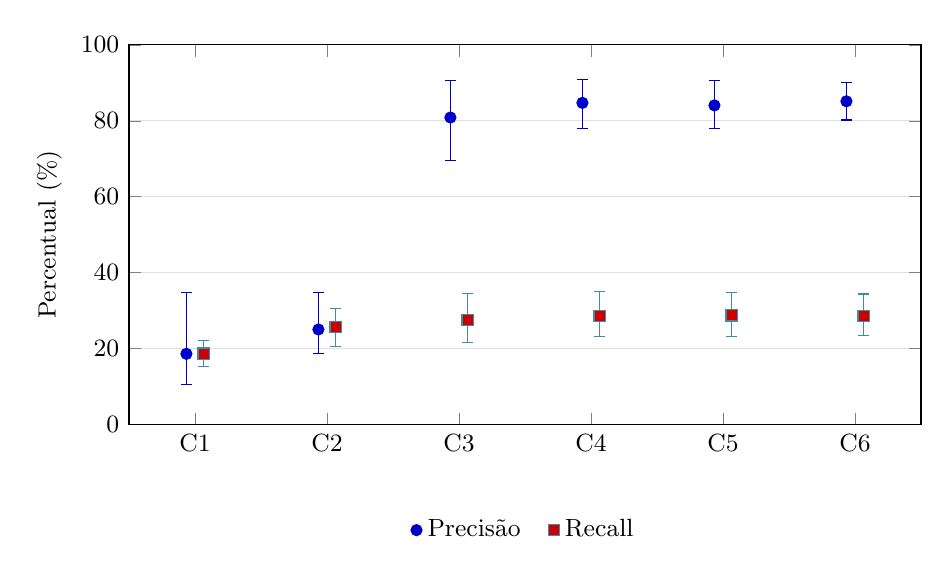
\begin{tikzpicture}
\begin{axis}[
width=0.96\textwidth,height=6.4cm,
tick label style={font=\small},label style={font=\small},
legend style={font=\small,at={(0.5,-0.22)},anchor=north,legend columns=3,draw=none,/tikz/every even column/.append style={column sep=8pt}},
ymajorgrids=true,grid style={black!12},
xmin=0.5,xmax=6.5,ymin=0,ymax=100,ylabel={Percentual (\%)},xtick={1,2,3,4,5,6},xticklabels={C1,C2,C3,C4,C5,C6}
]
\addplot+[only marks,mark=*,color=blue!75!black,error bars/.cd,y dir=both,y explicit] coordinates {(0.93500000,18.57142857) += (0,16.11708477) -= (0,8.07569674) (1.93500000,25.00000000) += (0,9.77092181) -= (0,6.22213370) (2.93500000,80.87164501) += (0,9.77396971) -= (0,11.33461896) (3.93500000,84.72830970) += (0,6.16940271) -= (0,6.64804791) (4.93500000,84.06008400) += (0,6.57338899) -= (0,6.07898575) (5.93500000,85.14619640) += (0,4.83511586) -= (0,4.94028284)};
\addlegendentry{Precisão}
\addplot+[only marks,mark=square*,color=cyan!65!black,error bars/.cd,y dir=both,y explicit] coordinates {(1.06500000,18.65136298) += (0,3.42665042) -= (0,3.51251962) (2.06500000,25.68149211) += (0,4.79917148) -= (0,5.13890883) (3.06500000,27.45098039) += (0,7.14032283) -= (0,5.84691576) (4.06500000,28.59875658) += (0,6.52716672) -= (0,5.35201077) (5.06500000,28.69440459) += (0,5.99957241) -= (0,5.49053828) (6.06500000,28.50310856) += (0,5.86078748) -= (0,5.15819372)};
\addlegendentry{Recall}
\end{axis}
\end{tikzpicture}

\legend{Fonte: Elaborado pelo autor a partir da avaliação (2026).}
\end{figure}

\begin{figure}[htbp]
\centering
\caption{\label{fig:fscores}F1, F2 e F3 por condição, com IC95\%}
% Gerado por scripts/gerar-figuras-monografia.py; não editar.
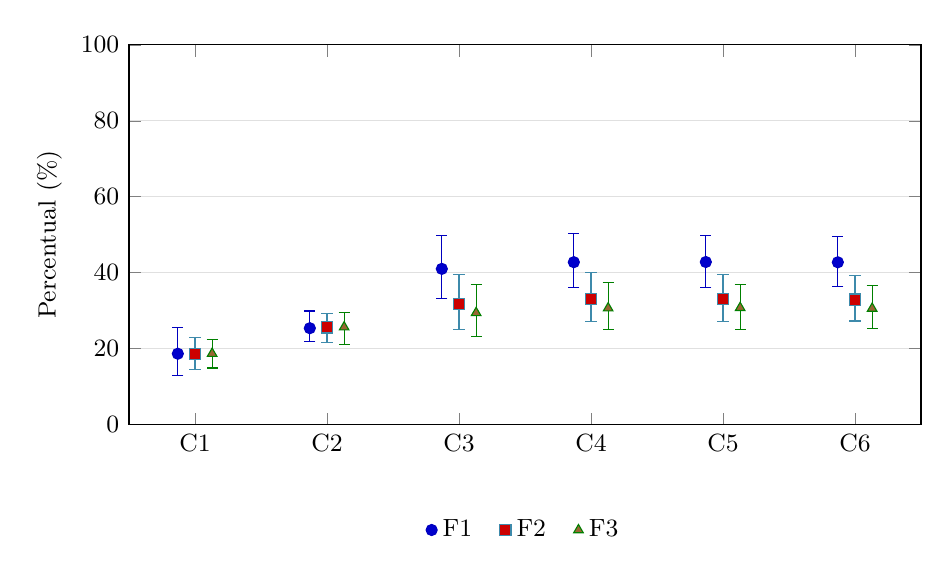
\begin{tikzpicture}
\begin{axis}[
width=0.96\textwidth,height=6.4cm,
tick label style={font=\small},label style={font=\small},
legend style={font=\small,at={(0.5,-0.22)},anchor=north,legend columns=3,draw=none,/tikz/every even column/.append style={column sep=8pt}},
ymajorgrids=true,grid style={black!12},
xmin=0.5,xmax=6.5,ymin=0,ymax=100,ylabel={Percentual (\%)},xtick={1,2,3,4,5,6},xticklabels={C1,C2,C3,C4,C5,C6}
]
\addplot+[only marks,mark=*,color=blue!75!black,error bars/.cd,y dir=both,y explicit] coordinates {(0.87000000,18.61130995) += (0,6.84722789) -= (0,5.82806814) (1.87000000,25.33616419) += (0,4.54544097) -= (0,3.49708373) (2.87000000,40.97274631) += (0,8.85153624) -= (0,7.84895709) (3.87000000,42.73658605) += (0,7.51450416) -= (0,6.72689828) (4.87000000,42.78332711) += (0,6.96783547) -= (0,6.68501769) (5.87000000,42.70850447) += (0,6.79307509) -= (0,6.35802298)};
\addlegendentry{F1}
\addplot+[only marks,mark=square*,color=cyan!65!black,error bars/.cd,y dir=both,y explicit] coordinates {(1.00000000,18.63532110) += (0,4.28348038) -= (0,4.22431777) (2.00000000,25.54223744) += (0,3.56837222) -= (0,3.89829204) (3.00000000,31.62493749) += (0,7.78065707) -= (0,6.55701657) (4.00000000,32.95869612) += (0,6.97497203) -= (0,5.84634722) (5.00000000,33.04749412) += (0,6.41306985) -= (0,5.98235441) (6.00000000,32.87723472) += (0,6.27838626) -= (0,5.63047293)};
\addlegendentry{F2}
\addplot+[only marks,mark=triangle*,color=green!50!black,error bars/.cd,y dir=both,y explicit] coordinates {(1.13000000,18.64333859) += (0,3.77820586) -= (0,3.79547747) (2.13000000,25.61167549) += (0,3.95023406) -= (0,4.49486770) (3.13000000,29.39041406) += (0,7.44156470) -= (0,6.18015840) (4.13000000,30.62416618) += (0,6.75413353) -= (0,5.59066194) (5.13000000,30.71748793) += (0,6.20526386) -= (0,5.74609793) (6.13000000,30.53431220) += (0,6.07288500) -= (0,5.38999896)};
\addlegendentry{F3}
\end{axis}
\end{tikzpicture}

\legend{Fonte: Elaborado pelo autor a partir da avaliação (2026).}
\end{figure}

\begin{table}[htb]
\ABNTEXfontereduzida
\caption{\label{tab:resultados-deteccao-condicao}Desempenho de detecção por condição experimental}
\centering
\resizebox{\textwidth}{!}{%
\begin{tabular}{lrrrrrrr}
\hline
\textbf{Condição} & \textbf{Precisão} & \textbf{Recall} & \textbf{F1} &
\textbf{F2} & \textbf{F3} & \textbf{IC95\% F3} & \textbf{Taxa de FP} \\
\hline
C1 & 18,6\% & 18,7\% & 18,6\% & 18,6\% & 18,6\% & [14,8\%; 22,4\%] & 82,8\% \\
C2 & 25,0\% & 25,7\% & 25,3\% & 25,5\% & 25,6\% & [21,1\%; 29,6\%] & 82,6\% \\
C3 & 80,9\% & 27,5\% & 41,0\% & 31,6\% & 29,4\% & [23,2\%; 36,8\%] & 27,4\% \\
C4 & 84,7\% & 28,6\% & 42,7\% & 33,0\% & 30,6\% & [25,0\%; 37,4\%] & 23,0\% \\
C5 & 84,1\% & 28,7\% & 42,8\% & 33,0\% & 30,7\% & [25,0\%; 36,9\%] & 24,3\% \\
C6 & 85,1\% & 28,5\% & 42,7\% & 32,9\% & 30,5\% & [25,1\%; 36,6\%] & 22,6\% \\
\hline
\end{tabular}}
\legend{Fonte: Elaborado pelo autor (2026). IC95\% obtido por bootstrap em nível de repositório.}
\end{table}

As condições baseadas em IA apresentaram precisão substancialmente maior e taxa de
falsos positivos menor que as linhas de base SAST. C4 obteve a maior precisão entre
as condições isoladas (84,7\%), enquanto C6 atingiu a maior precisão geral (85,1\%)
e a menor taxa de falsos positivos (22,6\%). Em contrapartida, o \textit{recall}
 médio permaneceu abaixo de 29\% em todas as condições. C5 obteve o maior valor médio de
\textit{recall} (28,7\%) e F3 (30,7\%), porém com diferenças pequenas em relação
a C3, C4 e C6. Assim, o principal contraste observado não é uma cobertura ampla,
mas uma troca entre o elevado número de alertas incorretos do SAST e a seleção mais
conservadora das condições de IA.

A Figura~\ref{fig:taxa-fp} apresenta a taxa de falsos positivos calculada pelo
avaliador oficial. Essa taxa não equivale a $1-\text{precisão}$: o benchmark
contabiliza como FP também os alertas sem correspondência, enquanto TN se
restringe às armadilhas seguras corretamente ignoradas. Assim, o denominador
$FP+TN$ não representa todas as regiões seguras do código, e a medida deve ser
interpretada segundo essa convenção do RealVuln.

\begin{figure}[htbp]
\centering
\caption{\label{fig:taxa-fp}Taxa de falsos positivos segundo a convenção do RealVuln, com IC95\%}
% Gerado por scripts/gerar-figuras-monografia.py; não editar.
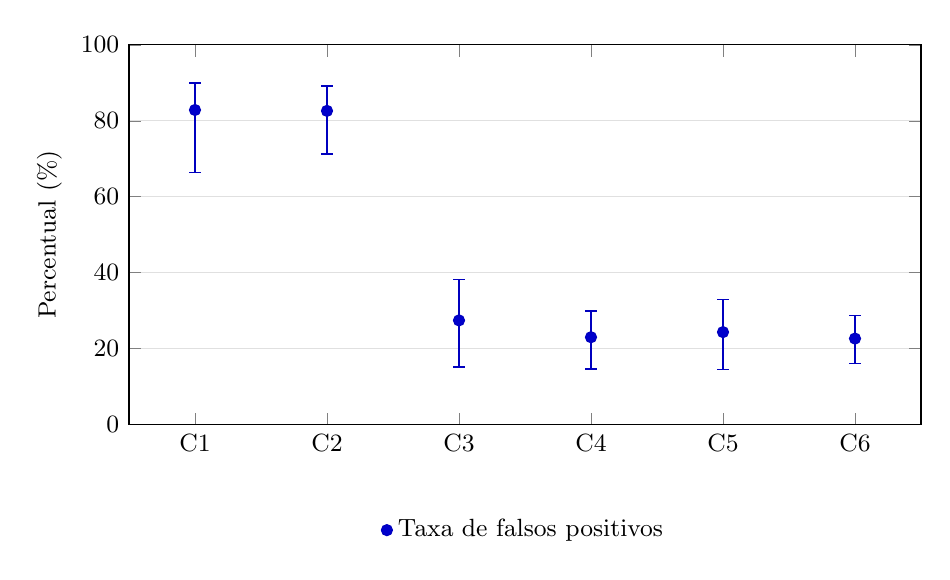
\begin{tikzpicture}
\begin{axis}[
width=0.96\textwidth,height=6.4cm,
tick label style={font=\small},label style={font=\small},
legend style={font=\small,at={(0.5,-0.22)},anchor=north,legend columns=3,draw=none,/tikz/every even column/.append style={column sep=8pt}},
ymajorgrids=true,grid style={black!12},
xmin=0.5,xmax=6.5,ymin=0,ymax=100,ylabel={Percentual (\%)},xtick={1,2,3,4,5,6},xticklabels={C1,C2,C3,C4,C5,C6}
]
\addplot+[only marks,mark=*,color=blue!75!black,error bars/.cd,y dir=both,y explicit] coordinates {(1.00000000,82.84883721) += (0,7.12111017) -= (0,16.50579514) (2.00000000,82.61538462) += (0,6.56855281) -= (0,11.35934597) (3.00000000,27.39170970) += (0,10.66985051) -= (0,12.26969440) (4.00000000,22.95877696) += (0,6.90046124) -= (0,8.38670716) (5.00000000,24.30522088) += (0,8.54667080) -= (0,9.79414146) (6.00000000,22.60480747) += (0,6.00662408) -= (0,6.66773359)};
\addlegendentry{Taxa de falsos positivos}
\end{axis}
\end{tikzpicture}

\legend{Fonte: Elaborado pelo autor a partir da avaliação (2026).}
\end{figure}

\subsection{Resultados por categoria CWE}\label{subsec:resultados-por-cwe}

A desagregação por famílias CWE mostrou forte dependência do tipo de vulnerabilidade.
Na categoria de injeção, o \textit{recall} variou de 35,5\% em C1 e 50,6\% em C2
até 56,6\%--64,7\% nas condições de IA, com o maior valor em C5. Para autenticação,
C1 e C2 alcançaram apenas 0,9\%, enquanto C3--C6 variaram de 22,0\% a 28,3\%.
Na categoria de sessão e configuração, C1 não detectou entradas, C2 alcançou 34,0\%
e as condições de IA permaneceram entre 6,4\% e 10,3\%. Os resultados completos
por CWE e repetição foram preservados nos artefatos de avaliação; categorias com
poucas entradas devem ser interpretadas descritivamente.

\subsection{Resultados por severidade}\label{subsec:resultados-por-severidade}

\begin{table}[htb]
\ABNTEXfontereduzida
\caption{\label{tab:recall-severidade}Recall por severidade de referência}
\centering
\begin{tabular}{lrrrr}
\hline
\textbf{Condição} & \textbf{Baixa} & \textbf{Média} & \textbf{Alta} & \textbf{Crítica} \\
\hline
C1 & 14,7\% & 10,8\% & 19,7\% & 44,2\% \\
C2 & 5,9\% & 22,6\% & 22,0\% & 62,8\% \\
C3 & 3,4\% & 15,1\% & 33,6\% & 67,8\% \\
C4 & 3,9\% & 17,7\% & 32,6\% & 71,3\% \\
C5 & 3,9\% & 14,6\% & 34,1\% & 77,5\% \\
C6 & 3,9\% & 15,3\% & 33,7\% & 74,8\% \\
\hline
\end{tabular}
\legend{Fonte: Elaborado pelo autor (2026). Nas condições C3--C6, valores médios das três repetições.}
\end{table}

O \textit{recall} cresceu com a severidade de referência. C5 detectou, em média,
77,5\% das vulnerabilidades críticas, mas somente 3,9\% das de severidade baixa.
Esse padrão favorece a descoberta das falhas de maior impacto, embora também mostre
que a cobertura global reduzida não se distribui uniformemente pelo corpus.

A Figura~\ref{fig:recall-severidade} permite comparar esse padrão entre condições.
As categorias são as severidades de referência do benchmark, e não as etiquetas
atribuídas pelas ferramentas.

\begin{figure}[htbp]
\centering
\caption{\label{fig:recall-severidade}Recall por severidade de referência}
% Gerado por scripts/gerar-figuras-monografia.py; não editar.
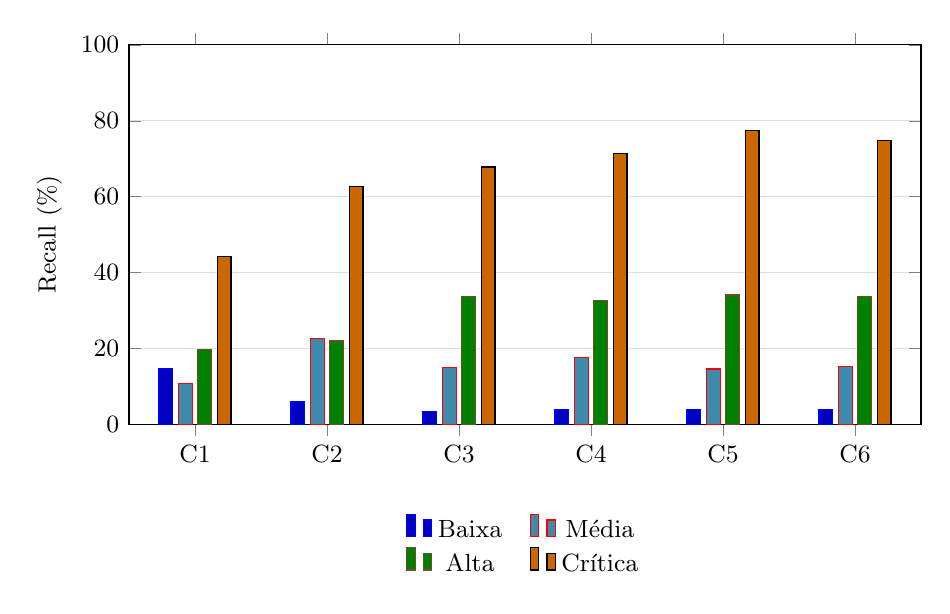
\begin{tikzpicture}
\begin{axis}[
width=0.96\textwidth,height=6.4cm,
tick label style={font=\small},label style={font=\small},
legend style={font=\small,at={(0.5,-0.22)},anchor=north,legend columns=3,draw=none,/tikz/every even column/.append style={column sep=8pt}},
ymajorgrids=true,grid style={black!12},
ybar,bar width=5pt,ymin=0,ymax=100,ylabel={Recall (\%)},xtick={1,2,3,4,5,6},xticklabels={C1,C2,C3,C4,C5,C6},enlarge x limits=0.1,legend columns=2
]
\addplot+[ybar,fill=blue!75!black] coordinates {(1,14.70588235) (2,5.88235294) (3,3.43137255) (4,3.92156863) (5,3.92156863) (6,3.92156863)};
\addlegendentry{Baixa}
\addplot+[ybar,fill=cyan!65!black] coordinates {(1,10.75268817) (2,22.58064516) (3,15.05376344) (4,17.68219833) (5,14.57586619) (6,15.29271207)};
\addlegendentry{Média}
\addplot+[ybar,fill=green!50!black] coordinates {(1,19.69696970) (2,21.96969697) (3,33.58585859) (4,32.57575758) (5,34.09090909) (6,33.71212121)};
\addlegendentry{Alta}
\addplot+[ybar,fill=orange!80!black] coordinates {(1,44.18604651) (2,62.79069767) (3,67.82945736) (4,71.31782946) (5,77.51937984) (6,74.80620155)};
\addlegendentry{Crítica}
\end{axis}
\end{tikzpicture}

\legend{Fonte: Elaborado pelo autor a partir da avaliação (2026). C3--C6: médias das três repetições.}
\end{figure}

\section{Qualidade dos Relatórios Verdadeiros-Positivos (QP2)}\label{sec:qualidade-relatorios}

\subsection{Amostra e estado da avaliação}\label{subsec:resultados-rubrica}

Foi preparada uma amostra cega conforme o protocolo. Foram
identificadas 35 entradas detectadas por todas as condições na primeira repetição;
20 foram sorteadas para o recorte comum. Em seguida, cada condição foi completada
até 50 relatórios por amostragem estratificada por CWE e severidade, totalizando
300 avaliações.

Os relatórios usam identificadores opacos, sem indicação da condição. A chave
de cegamento é mantida separada durante a pontuação. O recorte comum permite
comparar relatos das mesmas 20 vulnerabilidades; a amostra completa descreve
a utilidade dos verdadeiros positivos de cada condição, com composição própria.
Por se restringir aos achados associados à referência, esta avaliação não mede
a qualidade dos falsos positivos nem representa todos os relatórios emitidos.

A pontuação foi aplicada por um avaliador LLM de família distinta da usada nas
condições C3--C6, conforme a Seção~\ref{subsec:metricas-qualitativas-metodologia}.
O avaliador, o registro e a validação das pontuações estão descritos na
Seção~\ref{subsec:registro-pontuacao-qualitativa}.

\subsection{Procedimento de pontuação estruturada}\label{subsec:procedimento-pontuacao-qualitativa}

Após a análise quantitativa, os 300 relatórios foram pontuados por rubrica
explícita, aplicada por um modelo de linguagem como avaliador para tornar viável
a pontuação de toda a amostra. Essa etapa constitui uma extensão exploratória do
protocolo. Os escores são interpretados como julgamentos sobre o material
fornecido; não constituem confirmação por exploração dinâmica nem verdade de
referência sobre a qualidade dos relatos.

Cada relatório é examinado com sua descrição, recomendação, referência
específica do benchmark e trecho numerado do código sanitizado. A associação
quantitativa a um verdadeiro positivo não concede automaticamente a nota máxima
de correção ou localização. Afirmações sobre o mecanismo precisam ser
sustentadas pelo código ou pela referência; a posição reportada precisa apontar
o trecho causal. Quando o suporte é insuficiente, a dimensão recebe valor
ausente, acompanhado de justificativa.

\begin{table}[htbp]
\ABNTEXfontereduzida
\caption{\label{tab:rubrica-pontuacao-estruturada}Âncoras da pontuação estruturada dos relatórios}
\centering
\begin{tabularx}{\textwidth}{|l|X|X|X|}
\hline
\textbf{Dimensão} & \textbf{Nota 1} & \textbf{Nota 3} & \textbf{Nota 5} \\
\hline
Correção técnica & Mecanismo falso ou contradito pelo material & Classe e risco plausíveis, com explicação genérica ou ressalva relevante & Fonte, operação, pré-condição e consequência coerentes com o material \\
\hline
Localização & Arquivo ou operação contraditos & Região ou função correta, com ambiguidade & Instrução causal precisamente indicada \\
\hline
Acionabilidade & Orientação ausente ou solução insegura & Direção aplicável, com escolhas essenciais ausentes & Controle e mudança concretos, com condições suficientes de aplicação \\
\hline
\end{tabularx}
\legend{Fonte: Elaborado pelo autor (2026). Notas 2 e 4 representam posições intermediárias.}
\end{table}

A clareza compreende cinco itens binários: identificação do problema, risco
explícito, contexto técnico, concretude e concisão. Cada item recebe um ou zero,
com justificativa ligada ao texto. A pontuação considera o sentido do texto e
sua relação com o material de suporte.

O esquema \path{config/avaliacao-qualitativa/schema-julgamento.json} exige
identificador do relatório, notas, decisões dos
cinco itens, justificativas e referências ao material de suporte. Dimensões não
avaliáveis devem conter valor nulo e motivo de abstenção; registros incompletos
ou fora das escalas são rejeitados. A chave das condições somente é utilizada
para agregação depois do congelamento dos julgamentos.

Para sintetizar a rubrica, definiu-se um score de zero a cem com peso igual
de 25 pontos para cada dimensão. Sejam $T$, $L$ e $A$ as notas ordinais de
correção técnica, localização e acionabilidade, e $c_j$ os cinco itens de
clareza. O score é:
\begin{equation}
S = 25\left(\frac{T-1}{4}+\frac{L-1}{4}+\frac{A-1}{4}
      +\frac{\sum_{j=1}^{5}c_j}{5}\right).
\label{eq:score-qualitativo}
\end{equation}

Na ausência de qualquer dimensão, o score total permanece nulo, sem imputação
ou redistribuição dos pesos. A cobertura de pontuação é reportada junto aos
resultados. Os pesos foram fixados nesta etapa exploratória, antes dos
julgamentos qualitativos, mas após a análise quantitativa; não representam uma
escala com validade psicométrica demonstrada. A apresentação conserva também
as dimensões separadas, evitando reduzir a qualidade a uma única nota.

\subsection{Escores por condição}\label{subsec:resultados-escores-qualitativos}

\IfFileExists{figs/avaliacao/qualitativa-condicoes.tex}{%
A Tabela~\ref{tab:qualitativa-condicoes} apresenta, para os 50 relatos de cada
condição, a média de cada dimensão e do score entre os valores válidos. A
coluna de scores válidos indica quantos relatos tiveram as oito decisões
avaliáveis; as abstenções reduzem o número de valores de cada dimensão e não
são imputadas. Como a amostra é restrita a verdadeiros positivos e composta por
estratificação própria de cada condição, as médias descrevem os relatos
selecionados e não a qualidade de todos os alertas emitidos.

\begin{table}[htb]
\ABNTEXfontereduzida
\caption{\label{tab:qualitativa-condicoes}Pontuação média dos relatos verdadeiros-positivos por condição}
\centering
\resizebox{\textwidth}{!}{% Gerado por scripts/gerar-tabela-qualitativa.py; não editar.
\begin{tabular}{|l|r|r|r|r|r|r|r|}
\hline
\textbf{Condição} & \textbf{Relatos} & \textbf{Scores válidos} & \textbf{Correção} & \textbf{Localização} & \textbf{Acionabilidade} & \textbf{Clareza (0--5)} & \textbf{Score} \\
\hline
C1 & 50 & 50 & 3,20 & 4,64 & 1,30 & 3,00 & 53,38 \\
\hline
C2 & 50 & 50 & 3,64 & 4,74 & 3,28 & 4,22 & 75,22 \\
\hline
C3 & 50 & 50 & 4,76 & 4,14 & 4,60 & 5,00 & 90,62 \\
\hline
C4 & 50 & 50 & 4,76 & 3,62 & 4,68 & 5,00 & 87,88 \\
\hline
C5 & 50 & 50 & 4,84 & 4,56 & 4,56 & 5,00 & 93,50 \\
\hline
C6 & 50 & 50 & 4,82 & 4,60 & 4,64 & 5,00 & 94,12 \\
\hline
\end{tabular}
}
\legend{Fonte: Elaborado pelo autor a partir da pontuação qualitativa (2026). Correção, localização e acionabilidade: escala de 1 a 5; clareza: contagem de 0 a 5; score: 0 a 100.}
\end{table}

A Tabela~\ref{tab:qualitativa-deltas} restringe a comparação aos 20 grupos de
referência comuns às seis condições. Cada diferença é calculada dentro do mesmo
grupo, entre a condição híbrida e a respectiva condição isolada, e só entra na
média quando as duas pontuações são válidas. Com apenas 20 grupos, as
diferenças permanecem descritivas e não sustentam inferência sobre o efeito
dos alertas SAST na qualidade.

\begin{table}[htb]
\ABNTEXfontereduzida
\caption{\label{tab:qualitativa-deltas}Diferença média de pontuação no recorte comum}
\centering
\resizebox{\textwidth}{!}{% Gerado por scripts/gerar-tabela-qualitativa.py; não editar.
\begin{tabular}{|l|r|r|r|r|r|r|}
\hline
\textbf{Comparação} & \textbf{Pares válidos} & \textbf{Correção} & \textbf{Localização} & \textbf{Acionabilidade} & \textbf{Clareza (0--5)} & \textbf{Score} \\
\hline
C5$-$C3 & 20 de 20 & 0,05 & 0,75 & $-$0,20 & 0,00 & 3,75 \\
\hline
C6$-$C4 & 20 de 20 & 0,20 & 1,10 & $-$0,05 & 0,00 & 7,81 \\
\hline
\end{tabular}
}
\legend{Fonte: Elaborado pelo autor a partir da pontuação qualitativa (2026). Diferenças entre pares do mesmo grupo de referência.}
\end{table}

A Figura~\ref{fig:qualidade-score} resume o score médio por condição, na amostra
completa e no recorte comum, e a Figura~\ref{fig:qualidade-dimensoes} separa as
dimensões no recorte comum. Em ambas, a ordenação dos grupos de condições é a
mesma da Tabela~\ref{tab:qualitativa-condicoes}.

\begin{figure}[htbp]
\centering
\caption{\label{fig:qualidade-score}Score médio dos relatos verdadeiros-positivos por condição}
% Gerado por scripts/gerar-figuras-monografia.py; não editar.
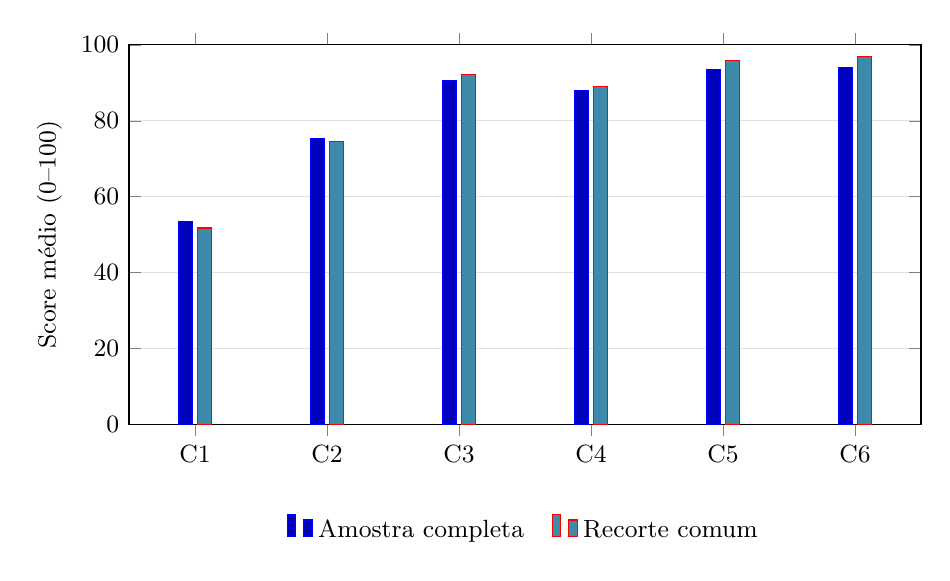
\begin{tikzpicture}
\begin{axis}[
width=0.96\textwidth,height=6.4cm,
tick label style={font=\small},label style={font=\small},
legend style={font=\small,at={(0.5,-0.22)},anchor=north,legend columns=3,draw=none,/tikz/every even column/.append style={column sep=8pt}},
ymajorgrids=true,grid style={black!12},
ybar,bar width=5pt,ymin=0,ymax=100,ylabel={Score médio (0--100)},xtick={1,2,3,4,5,6},xticklabels={C1,C2,C3,C4,C5,C6},enlarge x limits=0.1,legend columns=2
]
\addplot+[ybar,fill=blue!75!black] coordinates {(1,53.37500000) (2,75.22500000) (3,90.62500000) (4,87.87500000) (5,93.50000000) (6,94.12500000)};
\addlegendentry{Amostra completa}
\addplot+[ybar,fill=cyan!65!black] coordinates {(1,51.75000000) (2,74.62500000) (3,92.18750000) (4,89.06250000) (5,95.93750000) (6,96.87500000)};
\addlegendentry{Recorte comum}
\end{axis}
\end{tikzpicture}

\legend{Fonte: Elaborado pelo autor a partir da pontuação qualitativa (2026). Amostra completa: 50 relatos por condição; recorte comum: 20 grupos de referência.}
\end{figure}

\begin{figure}[htbp]
\centering
\caption{\label{fig:qualidade-dimensoes}Pontuação média por dimensão no recorte comum}
% Gerado por scripts/gerar-figuras-monografia.py; não editar.
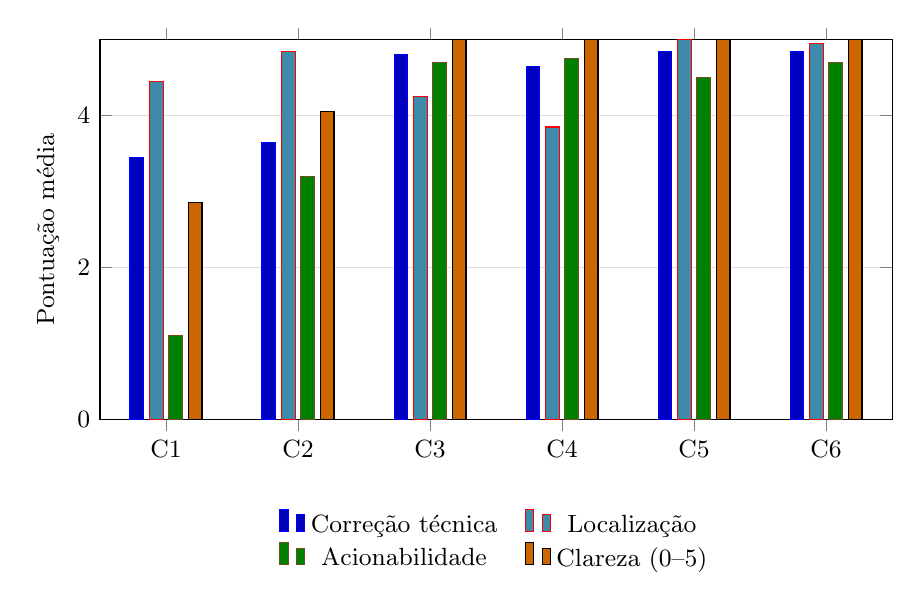
\begin{tikzpicture}
\begin{axis}[
width=0.96\textwidth,height=6.4cm,
tick label style={font=\small},label style={font=\small},
legend style={font=\small,at={(0.5,-0.22)},anchor=north,legend columns=3,draw=none,/tikz/every even column/.append style={column sep=8pt}},
ymajorgrids=true,grid style={black!12},
ybar,bar width=5pt,ymin=0,ymax=5,ylabel={Pontuação média},xtick={1,2,3,4,5,6},xticklabels={C1,C2,C3,C4,C5,C6},enlarge x limits=0.1,legend columns=2
]
\addplot+[ybar,fill=blue!75!black] coordinates {(1,3.45000000) (2,3.65000000) (3,4.80000000) (4,4.65000000) (5,4.85000000) (6,4.85000000)};
\addlegendentry{Correção técnica}
\addplot+[ybar,fill=cyan!65!black] coordinates {(1,4.45000000) (2,4.85000000) (3,4.25000000) (4,3.85000000) (5,5.00000000) (6,4.95000000)};
\addlegendentry{Localização}
\addplot+[ybar,fill=green!50!black] coordinates {(1,1.10000000) (2,3.20000000) (3,4.70000000) (4,4.75000000) (5,4.50000000) (6,4.70000000)};
\addlegendentry{Acionabilidade}
\addplot+[ybar,fill=orange!80!black] coordinates {(1,2.85000000) (2,4.05000000) (3,5.00000000) (4,5.00000000) (5,5.00000000) (6,5.00000000)};
\addlegendentry{Clareza (0--5)}
\end{axis}
\end{tikzpicture}

\legend{Fonte: Elaborado pelo autor a partir da pontuação qualitativa (2026). A clareza é a contagem de 0 a 5 itens atendidos; as demais dimensões usam a escala de 1 a 5.}
\end{figure}

Os escores médios foram menores nas condições SAST isoladas e maiores nas
condições com agentes de IA. Na amostra completa, o score médio foi de 53,4
para C1 e 75,2 para C2, contra 90,6 para C3, 87,9 para C4, 93,5 para C5 e 94,1
para C6; no recorte comum, os valores foram 51,8, 74,6, 92,2, 89,1, 95,9 e 96,9.
A diferença entre as famílias concentra-se na acionabilidade (1,30 em C1 e 3,28
em C2, contra 4,56 a 4,68 nas condições de IA), na correção técnica (3,20 e 3,64,
contra 4,76 a 4,84) e na clareza (3,00 e 4,22, contra 5,00). Uma explicação possível, não testada aqui, é que os alertas SAST trazem
mensagens curtas e, frequentemente, sem recomendação própria.

A localização apresentou o padrão inverso entre as condições isoladas: C1 e C2
tiveram médias de 4,64 e 4,74, enquanto C3 e C4 tiveram 4,14 e 3,62. Uma explicação possível, não testada aqui, é que as regras SAST apontam
diretamente a instrução sinalizada, ao passo que os agentes sem alertas por
vezes indicam a região ou a função correta sem a linha causal. As condições híbridas recuperaram essa
dimensão (4,56 em C5 e 4,60 em C6).

No recorte comum, a Tabela~\ref{tab:qualitativa-deltas} mostra que a diferença
de score entre a condição híbrida e a respectiva condição isolada foi de 3,75
pontos para C5$-$C3 e de 7,81 pontos para C6$-$C4. Essas diferenças vieram
sobretudo da localização (0,75 e 1,10 pontos na escala de 1 a 5), com variações
pequenas em correção técnica (0,05 e 0,20) e ligeiramente negativas em
acionabilidade ($-$0,20 e $-$0,05); a clareza não variou. Com 20 grupos e sem
intervalos inferenciais, esses valores são descritivos e não permitem afirmar
efeito dos alertas SAST na qualidade das explicações.

A clareza atingiu o valor máximo (cinco itens atendidos) em todos os relatos de
C3 a C6, o que indica efeito de teto: nessa dimensão, a rubrica não distingue as
condições de IA entre si. Os demais resultados também estão sujeitos aos limites
da etapa: a amostra contém apenas verdadeiros positivos, a composição difere
entre as condições, o cegamento é parcial pelo estilo dos textos, e as
pontuações provêm de um único avaliador LLM, sem calibração contra avaliadores
humanos. Os escores devem ser lidos como evidência exploratória sobre a
utilidade dos achados corretos, e não como medida da qualidade global das
ferramentas.
}{%
Os 300 julgamentos ainda não foram concluídos e congelados; por isso, esta
seção não apresenta médias, diferenças nem comparações entre condições. A
tabela por condição e a tabela do recorte comum são geradas por
\path{scripts/gerar-tabela-qualitativa.py} a partir do resumo congelado e
aparecem aqui quando esse arquivo existe. Nenhuma conclusão sobre a QP2 deve
ser derivada de tentativas parciais, nem da leitura de relatos isolados.
}

\section{Efeito da Combinação SAST + IA (QP3)}\label{sec:efeito-hibrido}

A comparação pareada entre C5 e C3 indicou diferenças médias de 1,24 ponto
percentual em \textit{recall} (IC95\%: $-3,26$ a 5,43), 1,33 ponto em F3
(IC95\%: $-3,36$ a 5,70), 3,19 pontos em precisão (IC95\%: $-1,62$ a 9,26)
e $-3,09$ pontos na taxa de falsos positivos (IC95\%: $-7,23$ a 2,38).

Entre C6 e C4, as diferenças foram $-0,10$ ponto em \textit{recall}
(IC95\%: $-3,01$ a 2,61), $-0,09$ ponto em F3
(IC95\%: $-3,12$ a 2,75), 0,42 ponto em precisão
(IC95\%: $-4,47$ a 5,64) e $-0,35$ ponto na taxa de falsos positivos
(IC95\%: $-5,57$ a 5,03).

Nenhum desses intervalos excluiu zero. Sob este corpus e estas configurações,
fornecer os alertas normalizados de Bandit e Semgrep não produziu evidência
quantitativa conclusiva de melhora ou degradação na detecção. O pequeno ganho
pontual observado para C5 deve ser tratado como descritivo, e não como confirmação
de vantagem do arranjo híbrido. Quanto à qualidade das explicações, a pontuação qualitativa
descreve diferenças de localização no recorte comum, discutidas na
Seção~\ref{subsec:resultados-escores-qualitativos}, sem inferência estatística.

A Figura~\ref{fig:comparacoes-pareadas} representa as diferenças de precisão,
\textit{recall} e F3. A linha em zero indica ausência de diferença; a inclusão
desse valor nos intervalos impede concluir uma vantagem a partir das estimativas
pontuais. Isso também não demonstra equivalência entre as condições.

\begin{figure}[htbp]
\centering
\caption{\label{fig:comparacoes-pareadas}Diferenças pareadas entre condições híbridas e isoladas, com IC95\%}
% Gerado por scripts/gerar-figuras-monografia.py; não editar.
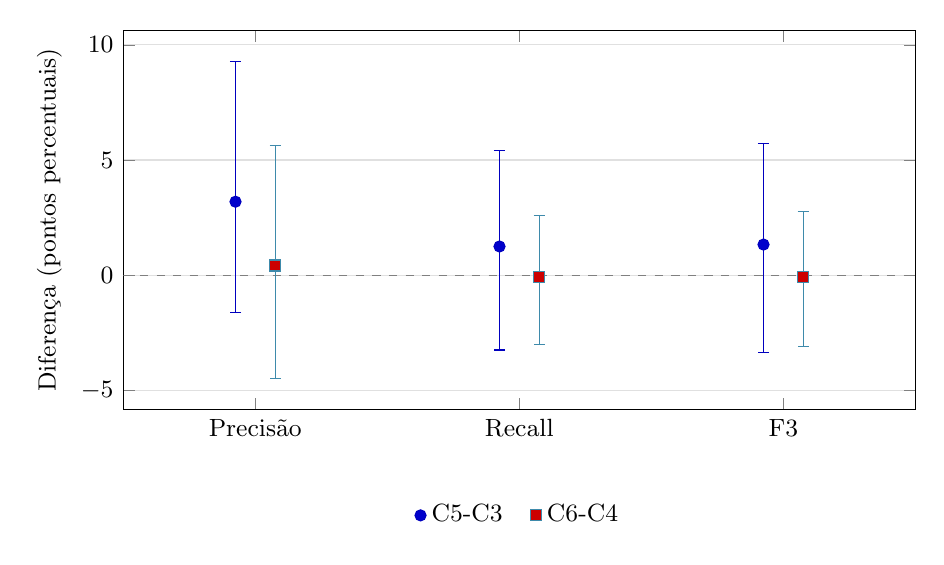
\begin{tikzpicture}
\begin{axis}[
width=0.96\textwidth,height=6.4cm,
tick label style={font=\small},label style={font=\small},
legend style={font=\small,at={(0.5,-0.22)},anchor=north,legend columns=3,draw=none,/tikz/every even column/.append style={column sep=8pt}},
ymajorgrids=true,grid style={black!12},
xmin=0.5,xmax=3.5,ylabel={Diferença (pontos percentuais)},xtick={1,2,3},xticklabels={Precisão,Recall,F3}
]
\addplot[black!50,dashed,forget plot] coordinates {(0.5,0) (3.5,0)};
\addplot+[only marks,color=blue!75!black,error bars/.cd,y dir=both,y explicit] coordinates {(0.92500000,3.18843898) += (0,6.07279336) -= (0,4.80556317) (1.92500000,1.24342420) += (0,4.18475529) -= (0,4.49905567) (2.92500000,1.32707387) += (0,4.37150277) -= (0,4.68422681)};
\addlegendentry{C5-C3}
\addplot+[only marks,color=cyan!65!black,error bars/.cd,y dir=both,y explicit] coordinates {(1.07500000,0.41788669) += (0,5.22151223) -= (0,4.89168737) (2.07500000,-0.09564802) += (0,2.70297448) -= (0,2.91229883) (3.07500000,-0.08985398) += (0,2.84265537) -= (0,3.02768540)};
\addlegendentry{C6-C4}
\end{axis}
\end{tikzpicture}

\legend{Fonte: Elaborado pelo autor a partir da avaliação (2026). Diferença: híbrida menos isolada.}
\end{figure}

\section{Estabilidade entre Execuções (QP4)}\label{sec:estabilidade-execucoes}

\begin{table}[htb]
\ABNTEXfontereduzida
\caption{\label{tab:estabilidade-resultados}Frequência de detecção das 697 vulnerabilidades nas três repetições}
\centering
\begin{tabular}{lrrrrrr}
\hline
\textbf{Condição} & \textbf{0 de 3} & \textbf{1 de 3} & \textbf{2 de 3} &
\textbf{3 de 3} & \textbf{DP F3} & \textbf{Amplitude F3} \\
\hline
C3 & 446 & 65 & 49 & 137 & 0,0027 & 0,0054 \\
C4 & 433 & 60 & 74 & 130 & 0,0308 & 0,0601 \\
C5 & 437 & 64 & 52 & 144 & 0,0095 & 0,0170 \\
C6 & 433 & 74 & 48 & 142 & 0,0017 & 0,0029 \\
\hline
\end{tabular}
\legend{Fonte: Elaborado pelo autor (2026). DP: desvio-padrão entre as métricas das três repetições.}
\end{table}

A maior parte das vulnerabilidades permaneceu sem detecção nas três execuções.
Entre as detectadas, C5 obteve o maior número de ocorrências consistentes
(144 entradas em três de três), seguido de C6 (142). C6 apresentou a menor
variação agregada de F3, enquanto C4 apresentou a maior. A análise por entrada
evidencia que métricas agregadas próximas podem ocultar variação na identidade
dos casos encontrados.

A Figura~\ref{fig:estabilidade-ia} mostra que a faixa de ausência de detecção
predomina em todas as condições. A estabilidade de uma métrica agregada deve,
portanto, ser distinguida da repetibilidade da identificação de cada falha.

\begin{figure}[htbp]
\centering
\caption{\label{fig:estabilidade-ia}Frequência de detecção das 697 vulnerabilidades nas três repetições}
% Gerado por scripts/gerar-figuras-monografia.py; não editar.
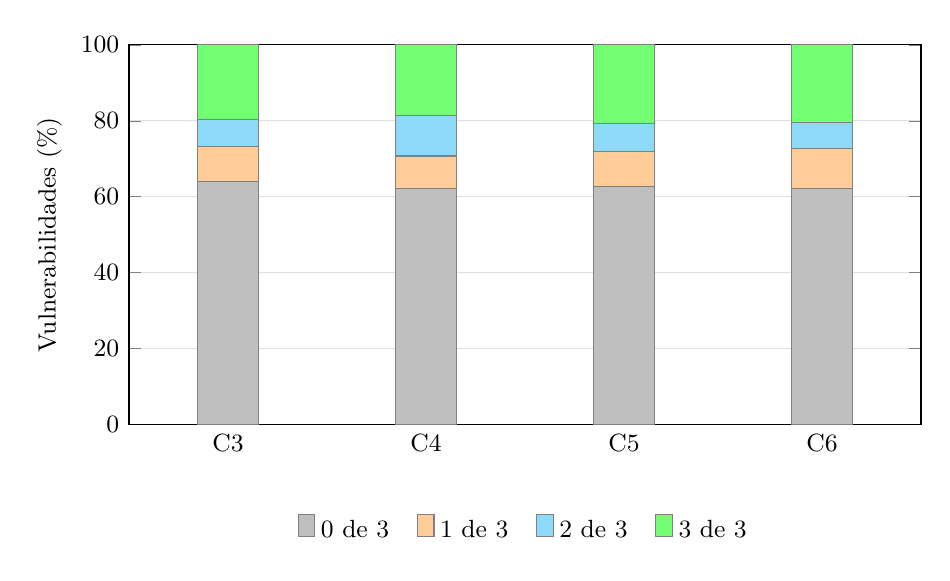
\begin{tikzpicture}
\begin{axis}[
width=0.96\textwidth,height=6.4cm,
tick label style={font=\small},label style={font=\small},
legend style={font=\small,at={(0.5,-0.22)},anchor=north,legend columns=3,draw=none,/tikz/every even column/.append style={column sep=8pt}},
ymajorgrids=true,grid style={black!12},
ybar stacked,bar width=22pt,xmin=0.5,xmax=4.5,ymin=0,ymax=100,ylabel={Vulnerabilidades (\%)},xtick={1,2,3,4},xticklabels={C3,C4,C5,C6},legend columns=4
]
\addplot+[fill=black!25,draw=black!50] coordinates {(1,63.98852224) (2,62.12338594) (3,62.69727403) (4,62.12338594)};
\addlegendentry{0 de 3}
\addplot+[fill=orange!40,draw=black!50] coordinates {(1,9.32568149) (2,8.60832138) (3,9.18220947) (4,10.61692970)};
\addlegendentry{1 de 3}
\addplot+[fill=cyan!45,draw=black!50] coordinates {(1,7.03012912) (2,10.61692970) (3,7.46054519) (4,6.88665710)};
\addlegendentry{2 de 3}
\addplot+[fill=green!55,draw=black!50] coordinates {(1,19.65566714) (2,18.65136298) (3,20.65997131) (4,20.37302726)};
\addlegendentry{3 de 3}
\end{axis}
\end{tikzpicture}

\legend{Fonte: Elaborado pelo autor a partir da avaliação (2026). Cada barra representa todo o conjunto vulnerável.}
\end{figure}

\section{Priorização e Indicação de Severidade (QP4)}\label{sec:priorizacao-resultados}

Todas as condições produziram severidade para 100\% dos verdadeiros positivos
associados. A concordância exata com a referência foi de 10,0\% em C1, 43,0\%
em C2 e variou entre 56,3\% e 60,1\% em C3--C6. Com tolerância de uma categoria,
os valores foram 54,6\% em C1, 85,5\% em C2 e 98,5\%--99,3\% nas condições
de IA. O Kappa ponderado foi 0,101 em C1, 0,252 em C2, 0,607 em C3,
0,600 em C4, 0,585 em C5 e 0,576 em C6. Assim, as condições de IA priorizaram
melhor os achados que efetivamente localizaram, mas o fornecimento dos alertas
SAST não aumentou a concordância de severidade.

A Figura~\ref{fig:priorizacao} compara a concordância exata e a tolerância de
uma categoria. Os percentuais se referem somente aos verdadeiros positivos
associados; não descrevem a priorização das vulnerabilidades não detectadas.

\begin{figure}[htbp]
\centering
\caption{\label{fig:priorizacao}Concordância da severidade dos verdadeiros positivos com a referência}
% Gerado por scripts/gerar-figuras-monografia.py; não editar.
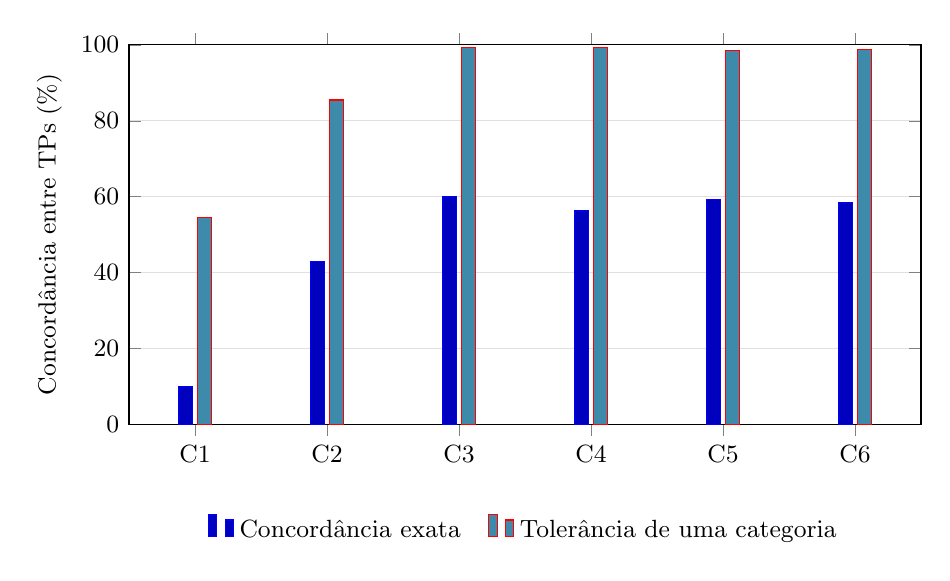
\begin{tikzpicture}
\begin{axis}[
width=0.96\textwidth,height=6.4cm,
tick label style={font=\small},label style={font=\small},
legend style={font=\small,at={(0.5,-0.22)},anchor=north,legend columns=3,draw=none,/tikz/every even column/.append style={column sep=8pt}},
ymajorgrids=true,grid style={black!12},
ybar,bar width=5pt,ymin=0,ymax=100,ylabel={Concordância entre TPs (\%)},xtick={1,2,3,4,5,6},xticklabels={C1,C2,C3,C4,C5,C6},enlarge x limits=0.1,legend columns=2
]
\addplot+[ybar,fill=blue!75!black] coordinates {(1,10.00000000) (2,43.01675978) (3,60.12295990) (4,56.34107541) (5,59.37188406) (6,58.56228956)};
\addlegendentry{Concordância exata}
\addplot+[ybar,fill=cyan!65!black] coordinates {(1,54.61538462) (2,85.47486034) (3,99.30094363) (4,99.33438593) (5,98.50066821) (6,98.82491582)};
\addlegendentry{Tolerância de uma categoria}
\end{axis}
\end{tikzpicture}

\legend{Fonte: Elaborado pelo autor a partir da avaliação (2026). C3--C6: médias das três repetições.}
\end{figure}

\section{Tempo de Execução e Consumo de Tokens}\label{sec:tempo-tokens-resultados}

\begin{table}[htb]
\ABNTEXfontereduzida
\caption{\label{tab:operacional-resultados}Mediana operacional por condição}
\centering
\begin{tabular}{lrrr}
\hline
\textbf{Condição} & \textbf{Mediana (s)} &
\textbf{IIQ (s)} & \textbf{Mínimo--máximo (s)} \\
\hline
C1 & 1,23 & [1,06; 1,58] & [0,73; 5,00] \\
C2 & 32,85 & [30,46; 35,74] & [27,91; 56,89] \\
C3 & 38,96 & [26,29; 46,26] & [11,15; 61,90] \\
C4 & 80,60 & [53,45; 96,23] & [11,05; 155,78] \\
C5 & 40,26 & [26,93; 48,28] & [13,92; 57,47] \\
C6 & 74,48 & [46,12; 96,18] & [15,51; 132,89] \\
\hline
\end{tabular}
\legend{Fonte: Elaborado pelo autor (2026). IIQ: intervalo interquartil.}
\end{table}

\begin{table}[htb]
\ABNTEXfontereduzida
\caption{\label{tab:tokens-resultados}Consumo de tokens informado nas condições de IA}
\centering
\begin{tabular}{lrrrr}
\hline
\textbf{Condição} & \textbf{Entrada mediana} & \textbf{Saída mediana} &
\textbf{Total mediano} & \textbf{IIQ do total} \\
\hline
C3 & 17.440,0 & 3.848,0 & 21.006,5 & [16.816,5; 26.340,3] \\
C4 & 19.955,0 & 3.980,5 & 23.433,5 & [19.814,0; 29.467,3] \\
C5 & 20.866,5 & 4.080,0 & 24.866,0 & [19.206,8; 30.328,3] \\
C6 & 23.259,5 & 4.000,5 & 27.436,5 & [21.839,3; 32.982,0] \\
\hline
\end{tabular}
\legend{Fonte: Elaborado pelo autor (2026). Cada condição possui 78 execuções com contadores disponíveis.}
\end{table}

C1 foi a condição mais rápida. Entre os agentes, as execuções Cursor (C3 e C5)
apresentaram menor mediana de tempo que as execuções Codex correspondentes
(C4 e C6). O contexto SAST aumentou a mediana de tokens em ambos os agentes,
mas não elevou de forma equivalente o tempo mediano. Como a contabilização de
tokens depende do produto, esses dados têm caráter operacional e descritivo.

As Figuras~\ref{fig:tempo-execucao} e~\ref{fig:tokens-ia} mostram mediana,
quartis e amplitude observada. As hastes vão do mínimo ao máximo, sem a regra de
1,5 intervalo interquartil utilizada em outros tipos de diagrama de caixa.
Os tempos e tokens referem-se às tentativas selecionadas, e não à soma de todas
as retentativas. Em C5 e C6, o tempo representa a chamada ao agente com os alertas
já disponíveis; não é a duração acumulada de C1, C2 e IA. Os dados não permitem
estimar custo monetário nem sustentar uma comparação de custo total entre produtos.

\begin{figure}[htbp]
\centering
\caption{\label{fig:tempo-execucao}Distribuição do tempo das tentativas selecionadas}
% Gerado por scripts/gerar-figuras-monografia.py; não editar.
\begin{tikzpicture}
\begin{axis}[
width=0.96\textwidth,height=6.4cm,
tick label style={font=\small},label style={font=\small},
legend style={font=\small,at={(0.5,-0.22)},anchor=north,legend columns=3,draw=none,/tikz/every even column/.append style={column sep=8pt}},
ymajorgrids=true,grid style={black!12},
boxplot/draw direction=y,ymin=0,ylabel={Tempo (segundos)},xtick={1,2,3,4,5,6},xticklabels={C1,C2,C3,C4,C5,C6},xmin=0.5,xmax=6.5
]
\addplot+[boxplot prepared={draw position=1,lower whisker=0.73283007,lower quartile=1.06195566,median=1.23184465,upper quartile=1.58002499,upper whisker=4.99905920},fill=blue!75!black,fill opacity=0.4,draw=black] coordinates {};
\addplot+[boxplot prepared={draw position=2,lower whisker=27.90629224,lower quartile=30.46044247,median=32.84519604,upper quartile=35.74433449,upper whisker=56.88560855},fill=cyan!65!black,fill opacity=0.4,draw=black] coordinates {};
\addplot+[boxplot prepared={draw position=3,lower whisker=11.14875700,lower quartile=26.29161600,median=38.96304200,upper quartile=46.26189600,upper whisker=61.89992500},fill=green!50!black,fill opacity=0.4,draw=black] coordinates {};
\addplot+[boxplot prepared={draw position=4,lower whisker=11.05069400,lower quartile=53.45327800,median=80.60136750,upper quartile=96.22751875,upper whisker=155.77710300},fill=orange!80!black,fill opacity=0.4,draw=black] coordinates {};
\addplot+[boxplot prepared={draw position=5,lower whisker=13.91961600,lower quartile=26.93426350,median=40.26267200,upper quartile=48.28402950,upper whisker=57.46941300},fill=red!65!black,fill opacity=0.4,draw=black] coordinates {};
\addplot+[boxplot prepared={draw position=6,lower whisker=15.51373000,lower quartile=46.12396550,median=74.48205100,upper quartile=96.18349275,upper whisker=132.88930700},fill=violet!80!black,fill opacity=0.4,draw=black] coordinates {};
\end{axis}
\end{tikzpicture}

\legend{Fonte: Elaborado pelo autor a partir da avaliação (2026). Caixa: Q1--Q3; linha: mediana; hastes: mínimo--máximo.}
\end{figure}

\begin{figure}[htbp]
\centering
\caption{\label{fig:tokens-ia}Distribuição dos tokens totais informados nas condições de IA}
% Gerado por scripts/gerar-figuras-monografia.py; não editar.
\begin{tikzpicture}
\begin{axis}[
width=0.96\textwidth,height=6.4cm,
tick label style={font=\small},label style={font=\small},
legend style={font=\small,at={(0.5,-0.22)},anchor=north,legend columns=3,draw=none,/tikz/every even column/.append style={column sep=8pt}},
ymajorgrids=true,grid style={black!12},
boxplot/draw direction=y,ymin=0,ylabel={Tokens totais informados},xtick={1,2,3,4},xticklabels={C3,C4,C5,C6},xmin=0.5,xmax=4.5
]
\addplot+[boxplot prepared={draw position=1,lower whisker=10826.00000000,lower quartile=16816.50000000,median=21006.50000000,upper quartile=26340.25000000,upper whisker=93314.00000000},fill=green!50!black,fill opacity=0.4,draw=black] coordinates {};
\addplot+[boxplot prepared={draw position=2,lower whisker=13446.00000000,lower quartile=19814.00000000,median=23433.50000000,upper quartile=29467.25000000,upper whisker=94391.00000000},fill=orange!80!black,fill opacity=0.4,draw=black] coordinates {};
\addplot+[boxplot prepared={draw position=3,lower whisker=12053.00000000,lower quartile=19206.75000000,median=24866.00000000,upper quartile=30328.25000000,upper whisker=110453.00000000},fill=red!65!black,fill opacity=0.4,draw=black] coordinates {};
\addplot+[boxplot prepared={draw position=4,lower whisker=14429.00000000,lower quartile=21839.25000000,median=27436.50000000,upper quartile=32982.00000000,upper whisker=112465.00000000},fill=violet!80!black,fill opacity=0.4,draw=black] coordinates {};
\end{axis}
\end{tikzpicture}

\legend{Fonte: Elaborado pelo autor a partir da avaliação (2026). Caixa: Q1--Q3; linha: mediana; hastes: mínimo--máximo.}
\end{figure}

\section{Discussão Integrada}\label{sec:discussao-integrada}

Os resultados respondem à QP1 mostrando que os agentes, isolados ou híbridos,
trocaram cobertura por seletividade: produziram precisão entre 80,9\% e 85,1\%
e taxa de falsos positivos entre 22,6\% e 27,4\%, mas não ultrapassaram 28,7\%
de \textit{recall}. As linhas de base SAST alcançaram precisão de até 25,0\%
e taxa de falsos positivos de pelo menos 82,6\%. A leitura por severidade, entretanto,
mostrou cobertura bem maior para vulnerabilidades críticas.

Quanto à QP3, as diferenças pareadas não sustentam uma vantagem geral da combinação
SAST + IA para detecção. O arranjo híbrido pode alterar quais entradas são
encontradas e aumentar o consumo de tokens, mas seus ganhos pontuais ficaram
dentro dos intervalos compatíveis com zero. Para a QP4, a estabilidade foi
heterogênea: C6 variou pouco em F3 agregado, embora nenhuma condição tenha
detectado consistentemente a maioria das vulnerabilidades. A priorização de
severidade foi mais próxima da referência nas condições de IA que no SAST.
Para a QP2, os relatos verdadeiros-positivos das condições de IA receberam
escores médios entre 87,9 e 94,1, contra 53,4 em C1 e 75,2 em C2, sobretudo por
acionabilidade, correção técnica e clareza; a localização, ao contrário, foi
menor em C3 e C4 que nas condições SAST. Na parte qualitativa da QP3, os
alertas SAST recuperaram a localização nas condições híbridas. Essas respostas
baseiam-se na pontuação cega da rubrica por um único avaliador LLM e, por isso,
são exploratórias.

\section{Ameaças à Validade Observadas na Coleta}\label{sec:ameacas-validade-observadas}

O uso do avaliador oficial e a preservação de seus arquivos por hash reduziram
o risco de divergência de pontuação. Ainda assim, o resultado depende das regras
de equivalência de CWE e da tolerância de localização do benchmark. A alta
densidade de vulnerabilidades do RealVuln impede extrapolar diretamente precisão
e prevalência para projetos de produção.

As tentativas operacionais repetidas foram tratadas por uma regra determinística
aplicada antes da consulta ao oráculo. Em C4, algumas respostas exigiram novas
tentativas por problemas de execução; o manifesto preserva esse histórico.
O identificador detalhado do modelo não estava presente em todos os registros
JSONL do produto, limitando a verificação independente além da configuração
declarada durante a coleta.

O não determinismo permaneceu visível mesmo com sessões independentes e
configurações controladas. Os intervalos de confiança preservam o agrupamento
por repositório, mas 26 projetos ainda representam um número limitado de
unidades independentes. O bloco complementar não executado restringe as
conclusões ao GPT-5.6 Luna e às versões e configurações registradas.

Por fim, a documentação de referência do RealVuln apresenta formulações
divergentes sobre F2 e F3 como métrica principal. Para evitar uma escolha
posterior aos resultados, esta avaliação manteve ambas as métricas implementadas
no avaliador oficial e adotou F3 como preestabelecido na metodologia. A etapa
qualitativa depende de julgamentos orientados pela rubrica. O cegamento e os
descritores explícitos reduzem, mas não eliminam, a subjetividade.

O estilo dos textos pode revelar sua origem, o que torna o cegamento parcial. A
verificação automática dos registros garante o formato, a coerência do score e a
presença de evidências e do material citado, mas não demonstra que a nota é
correta. O uso de um avaliador LLM de família distinta reduz o risco de
autopreferência \cite{Panickssery2024SelfPreference}, mas não elimina vieses
próprios desse tipo de avaliador, como a preferência por textos mais longos ou
mais detalhados \cite{Zheng2023LLMJudge}. Esse efeito pode favorecer os relatos
das condições de IA, mais extensos que as mensagens SAST, e a concordância das
notas com avaliadores humanos não foi medida neste trabalho.
